\documentclass[11pt,a4paper]{article}

% ========== Packages ==========
\usepackage[margin=2.5cm]{geometry}
\usepackage{amsmath,amssymb,bm}
\usepackage{graphicx}
\usepackage{hyperref}
\usepackage{cleveref}
\usepackage{algorithm2e}
\usepackage{booktabs}
\usepackage{enumitem}
\usepackage{tikz}
\usetikzlibrary{positioning, arrows.meta, calc, fit, backgrounds}
\usepackage{xcolor}

% ========== Custom commands ==========
\newcommand{\state}{\bm{x}}
\newcommand{\meas}{\bm{z}}
\newcommand{\resid}{\bm{r}}
\newcommand{\jac}{\bm{J}}
\newcommand{\hess}{\bm{H}}
\newcommand{\eye}{\bm{I}}
\newcommand{\cov}{\bm{\Sigma}}
\newcommand{\info}{\bm{\Lambda}}
\newcommand{\R}{\mathbb{R}}
\newcommand{\argmin}{\operatornamewithlimits{argmin}}
\newcommand{\norm}[1]{\left\| #1 \right\|}
\newcommand{\mahal}[2]{\left\| #1 \right\|^{2}_{#2}}
\DeclareMathOperator{\diag}{diag}
\DeclareMathOperator{\blkdiag}{blkdiag}

\title{\textbf{Factor Graph Optimisation for Sensor Fusion} \\[6pt]
       \large Theory, Application to Camera--Radar Target Tracking,\\
       and MATLAB Implementation}
\author{}
\date{}

\begin{document}
\maketitle

\tableofcontents
\newpage

% ######################################################################
\section{Introduction}
\label{sec:intro}
% ######################################################################

State estimation---the problem of recovering hidden quantities from noisy
measurements---lies at the heart of robotics, navigation, and target
tracking.  The two dominant paradigms are:

\begin{enumerate}
  \item \textbf{Sequential (recursive) filters}, such as the Extended
        Kalman Filter (EKF) and the Error-State Kalman Filter (ESKF),
        which process measurements one-at-a-time and maintain a single
        running estimate.
  \item \textbf{Batch (smoothing) methods}, which collect all
        measurements and optimise over the entire state trajectory at
        once.  \emph{Factor Graph Optimisation (FGO)} is the modern
        framework for formulating and solving such batch problems.
\end{enumerate}

This document provides a self-contained introduction to FGO with the
following goals:
\begin{itemize}[nosep]
  \item Present the general theory: probabilistic background, factor
        graphs, and Gauss--Newton optimisation.
  \item Apply the theory to a concrete problem: estimating a
        manoeuvring target's position and velocity from camera and radar
        measurements (the same problem solved by the existing ESKF
        implementation).
  \item Describe the companion MATLAB implementation in detail.
  \item Compare batch FGO with sequential ESKF conceptually.
\end{itemize}

\subsection*{Why Factor Graphs?}
Compared to sequential filtering, batch FGO offers several advantages:
\begin{itemize}[nosep]
  \item \textbf{Re-linearisation}: iterative optimisation can re-linearise
        at improved operating points, reducing linearisation error.
  \item \textbf{Delayed measurements}: a delayed sensor reading is simply
        attached to the correct past variable node---no special
        ``re-propagation'' or ``extrapolation'' mechanism is needed.
  \item \textbf{Loop closures}: constraints between non-adjacent time
        steps (e.g.\ revisiting a location) are handled naturally.
  \item \textbf{Sparsity}: the resulting optimisation problem has a
        sparse, banded structure that can be solved in linear time using
        sparse Cholesky factorisation.
\end{itemize}

The price is higher memory usage (all states are stored) and the fact
that the full solution is available only after all data have been
collected (though sliding-window variants exist for real-time use).

% ######################################################################
\section{Probabilistic Background}
\label{sec:background}
% ######################################################################

\subsection{Maximum a Posteriori (MAP) Estimation}

Let $\state_{0:K} = \{\state_0, \state_1, \ldots, \state_K\}$ denote the
collection of hidden states at discrete time steps, and let
$\meas_{1:K}$ denote all measurements.  We seek the \emph{MAP estimate}:
\begin{equation}
  \state_{0:K}^{*}
  = \argmin_{\state_{0:K}} \; -\log p(\state_{0:K} \mid \meas_{1:K}).
  \label{eq:map}
\end{equation}
By Bayes' rule, the posterior factorises as:
\begin{equation}
  p(\state_{0:K} \mid \meas_{1:K})
  \;\propto\;
  \underbrace{p(\state_0)}_{\text{prior}}
  \;\prod_{k=1}^{K}
  \underbrace{p(\state_k \mid \state_{k-1})}_{\text{dynamics}}
  \;\prod_{k \in \mathcal{C}}
  \underbrace{p(\meas_k^{\text{cam}} \mid \state_k)}_{\text{camera}}
  \;\prod_{k \in \mathcal{R}}
  \underbrace{p(\meas_k^{\text{rad}} \mid \state_k)}_{\text{radar}},
  \label{eq:factorisation}
\end{equation}
where $\mathcal{C}$ and $\mathcal{R}$ are the sets of time indices with
camera and radar measurements, respectively.

\subsection{From MAP to Nonlinear Least Squares}
\label{sec:map_to_nls}

If every factor in \eqref{eq:factorisation} is Gaussian:
\begin{equation}
  p(\bm{e}) \propto \exp\!\bigl(-\tfrac{1}{2}\,\bm{e}^{\!\top}
  \cov^{-1}\bm{e}\bigr),
  \qquad
  \bm{e} = \meas - h(\state)
  \;\;\text{or}\;\;
  \bm{e} = \state_k - f(\state_{k-1}),
\end{equation}
then taking $-\log$ of \eqref{eq:factorisation} yields a sum of squared
Mahalanobis norms:
\begin{equation}
  \boxed{
  \state_{0:K}^{*}
  = \argmin_{\state_{0:K}}
  \sum_{i} \mahal{\resid_i(\state_{0:K})}{\cov_i^{-1}}
  }
  \label{eq:nls}
\end{equation}
where $\mahal{\resid}{\cov^{-1}} \triangleq \resid^{\!\top}\cov^{-1}\resid$
is the squared Mahalanobis distance, and each $\resid_i$ is a \emph{residual
function} associated with one probabilistic factor.

This is a \textbf{nonlinear least-squares} (NLS) problem.

% ######################################################################
\section{Factor Graphs}
\label{sec:factor_graphs}
% ######################################################################

A \emph{factor graph} is a bipartite graph $G = (V, F, E)$ with two
types of nodes:

\begin{description}[nosep]
  \item[Variable nodes] $V = \{\state_0, \state_1, \ldots, \state_K\}$,
        representing the unknown states (drawn as circles).
  \item[Factor nodes] $F = \{f_0, f_1, \ldots\}$, representing
        probabilistic constraints/measurements (drawn as filled
        squares).
\end{description}

An edge connects factor $f_i$ to variable $\state_k$ if and only if
$\resid_i$ depends on $\state_k$.

\begin{figure}[htbp]
\centering
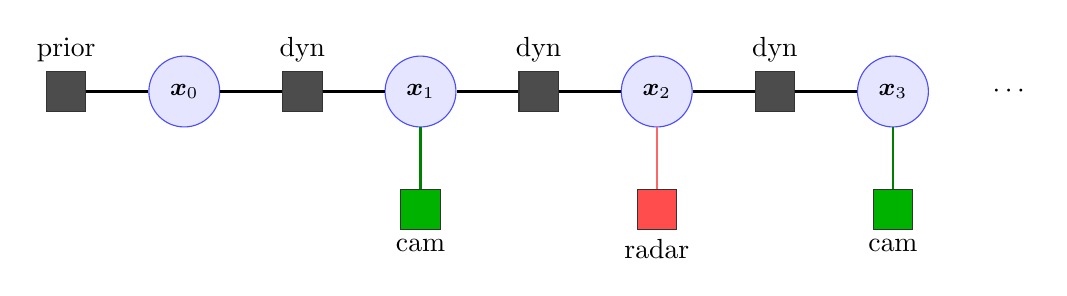
\begin{tikzpicture}[
    var/.style={circle, draw=blue!70, fill=blue!10, minimum size=9mm,
                font=\small},
    fac/.style={rectangle, draw=black!80, fill=black!70, minimum size=5mm,
                inner sep=0pt},
    edge/.style={thick},
    >=Stealth
  ]
  % Variable nodes
  \node[var] (x0) at (0,0) {$\state_0$};
  \node[var] (x1) at (3,0) {$\state_1$};
  \node[var] (x2) at (6,0) {$\state_2$};
  \node[var] (x3) at (9,0) {$\state_3$};
  \node at (10.5,0) {$\cdots$};

  % Prior factor
  \node[fac, label=above:{prior}] (fp) at (-1.5,0) {};
  \draw[edge] (fp) -- (x0);

  % Dynamics factors
  \node[fac, label=above:{dyn}] (f01) at (1.5,0) {};
  \node[fac, label=above:{dyn}] (f12) at (4.5,0) {};
  \node[fac, label=above:{dyn}] (f23) at (7.5,0) {};
  \draw[edge] (x0) -- (f01) -- (x1);
  \draw[edge] (x1) -- (f12) -- (x2);
  \draw[edge] (x2) -- (f23) -- (x3);

  % Camera factors
  \node[fac, fill=green!70!black, label=below:{cam}] (fc1) at (3,-1.5) {};
  \node[fac, fill=green!70!black, label=below:{cam}] (fc3) at (9,-1.5) {};
  \draw[edge, green!50!black] (fc1) -- (x1);
  \draw[edge, green!50!black] (fc3) -- (x3);

  % Radar factor
  \node[fac, fill=red!70, label=below:{radar}] (fr2) at (6,-1.5) {};
  \draw[edge, red!60] (fr2) -- (x2);
\end{tikzpicture}
\caption{Example factor graph for the target tracking problem.
         Variable nodes (circles) represent target states at discrete
         times.  Factor nodes (squares) encode constraints: prior
         (black), dynamics (black), camera (green), radar (red).}
\label{fig:factor_graph}
\end{figure}

\subsection{Common Factor Types}

\paragraph{Prior factor.}  Encodes initial knowledge about a variable:
$\resid_{\text{prior}} = \state_0 - \bm{\mu}_0$, with covariance
$\cov_0$.

\paragraph{Between (dynamics) factor.}  Connects two consecutive
variables via a motion model $f$:
$\resid_{\text{dyn}} = \state_{k+1} - f(\state_k)$, with process noise
covariance $\cov_w$.

\paragraph{Unary measurement factor.}  Relates a single variable to a
sensor reading via a measurement model $h$:
$\resid_{\text{meas}} = \meas_k - h(\state_k)$, with measurement noise
covariance $\cov_n$.

% ######################################################################
\section{Gauss--Newton Optimisation}
\label{sec:gauss_newton}
% ######################################################################

The NLS problem \eqref{eq:nls} is generally nonlinear.  We solve it
iteratively using the \textbf{Gauss--Newton (GN)} algorithm.

\subsection{Linearisation}

At the current estimate $\state^{(j)}$, we linearise each residual:
\begin{equation}
  \resid_i(\state^{(j)} + \delta\state)
  \;\approx\;
  \resid_i(\state^{(j)}) + \jac_i\,\delta\state,
  \qquad
  \jac_i = \frac{\partial \resid_i}{\partial \state}
           \bigg|_{\state^{(j)}}.
  \label{eq:linearise}
\end{equation}
Substituting into \eqref{eq:nls} and differentiating with respect to
$\delta\state$ gives the \textbf{normal equations}:
\begin{equation}
  \boxed{
  \hess\;\delta\state^{*} = \bm{b}
  }
  \label{eq:normal}
\end{equation}
where
\begin{align}
  \hess &= \sum_{i} \jac_i^{\!\top}\,\cov_i^{-1}\,\jac_i
          \qquad\text{(approximate Hessian / information matrix)},
  \label{eq:H} \\
  \bm{b} &= -\sum_{i} \jac_i^{\!\top}\,\cov_i^{-1}\,\resid_i
          \qquad\text{(right-hand side)}.
  \label{eq:b}
\end{align}

\subsection{Whitened Form}

Pre-multiplying each factor by $\cov_i^{-1/2}$ (the square root of the
information matrix):
\begin{equation}
  \tilde{\resid}_i = \cov_i^{-1/2}\,\resid_i,
  \qquad
  \tilde{\jac}_i = \cov_i^{-1/2}\,\jac_i,
\end{equation}
simplifies the normal equations to $\tilde{\jac}^{\!\top}\tilde{\jac}\;\delta\state
= -\tilde{\jac}^{\!\top}\tilde{\resid}$, which is a standard
unweighted least-squares problem solvable by sparse QR or Cholesky.

\subsection{GN Iteration}

\begin{algorithm}[H]
\SetAlgoLined
\KwIn{Initial estimate $\state^{(0)}$, tolerance $\epsilon$}
\For{$j = 0, 1, 2, \ldots$}{
  Evaluate all $\resid_i(\state^{(j)})$ and $\jac_i(\state^{(j)})$\;
  Build $\hess$ and $\bm{b}$ from \eqref{eq:H}--\eqref{eq:b}\;
  Solve $\hess\;\delta\state = \bm{b}$\;
  Update: $\state^{(j+1)} \leftarrow \state^{(j)} + \delta\state$\;
  \If{$\norm{\delta\state} < \epsilon$}{
    \textbf{return} $\state^{(j+1)}$\;
  }
}
\caption{Gauss--Newton Optimisation}
\label{alg:gn}
\end{algorithm}

\subsection{Sparse Structure}
\label{sec:sparsity}

Because each factor connects at most two consecutive variables, the
Hessian~$\hess$ has a \emph{block-tridiagonal} structure for chain-like
factor graphs.  This allows the linear system $\hess\,\delta\state =
\bm{b}$ to be solved in $O(K)$ time via sparse Cholesky factorisation,
where $K$ is the number of variable nodes.

\subsection{Levenberg--Marquardt Damping}
\label{sec:lm}

For improved robustness, a Levenberg--Marquardt (LM) damping term can be
added:
\begin{equation}
  (\hess + \lambda\,\eye)\;\delta\state = \bm{b},
\end{equation}
where $\lambda > 0$ interpolates between Gauss--Newton ($\lambda
\to 0$) and gradient descent ($\lambda \to \infty$).  This ensures
positive definiteness of the system matrix and controls the step size.

% ######################################################################
\section{Application: Visual--Radar Target Tracking}
\label{sec:application}
% ######################################################################

We now apply the general FGO framework to the same target-tracking
problem solved by the reduced ESKF.

\subsection{Problem Statement}

An interceptor equipped with a monocular camera and a radar sensor
observes a manoeuvring target.  The interceptor's own pose
$(\bm{R}^b_e(t),\, \bm{p}_I(t),\, \bm{v}_I(t))$ is assumed known
(from on-board navigation).  The goal is to estimate the target's
inertial position $\bm{p}_T$ and velocity $\bm{v}_T$ over time.

\subsection{State Definition}

At each discrete time $t_k$ we define a variable node:
\begin{equation}
  \state_k
  = \begin{bmatrix} \bm{p}_T^{(k)} \\ \bm{v}_T^{(k)} \end{bmatrix}
  \in \R^{6}.
  \label{eq:state_def}
\end{equation}

\begin{quote}
\emph{Note:} Unlike the ESKF, normalised image coordinates $\bar{\bm{p}}$
are \textbf{not} included in the state.  In batch FGO, $\bar{\bm{p}}$
is a deterministic function of $\bm{p}_T$ and the known interceptor
pose, so it need not be estimated separately.  This reduces the state
dimension from~8 (ESKF) to~6 (FGO).
\end{quote}

\subsection{Prior Factor}
\label{sec:prior}

The prior encodes initial knowledge about the target:
\begin{equation}
  \resid_{\text{prior}}(\state_0)
  = \state_0 - \bm{\mu}_0,
  \qquad
  \cov_{\text{prior}} = \diag(\sigma_{p}^{2}\eye_3,\;
                              \sigma_{v}^{2}\eye_3).
\end{equation}
The Jacobian is trivially the identity:
\begin{equation}
  \jac_{\text{prior}} = \frac{\partial \resid_{\text{prior}}}
                              {\partial \state_0} = \eye_6.
\end{equation}

\subsection{Dynamics Factor (Constant Velocity)}
\label{sec:dynamics}

We model the target with constant-velocity dynamics perturbed by
acceleration noise $\bm{w}_k \sim \mathcal{N}(\bm{0}, \bm{Q}_c)$:
\begin{equation}
  \bm{p}_T^{(k+1)} = \bm{p}_T^{(k)} + \bm{v}_T^{(k)}\,\Delta t,
  \qquad
  \bm{v}_T^{(k+1)} = \bm{v}_T^{(k)} + \bm{w}_k\,\Delta t.
  \label{eq:cv_model}
\end{equation}
In compact form, the prediction function is:
\begin{equation}
  f(\state_k) = \begin{bmatrix} \bm{p}_T^{(k)} + \bm{v}_T^{(k)}\Delta t \\
                                 \bm{v}_T^{(k)} \end{bmatrix}.
\end{equation}

\paragraph{Residual.}
\begin{equation}
  \resid_{\text{dyn}}(\state_k, \state_{k+1})
  = \state_{k+1} - f(\state_k).
\end{equation}

\paragraph{Jacobians.}
\begin{equation}
  \frac{\partial \resid_{\text{dyn}}}{\partial \state_k}
  = -\frac{\partial f}{\partial \state_k}
  = -\begin{bmatrix} \eye_3 & \Delta t\,\eye_3 \\
                      \bm{0}_3 & \eye_3 \end{bmatrix},
  \qquad
  \frac{\partial \resid_{\text{dyn}}}{\partial \state_{k+1}}
  = \eye_6.
  \label{eq:dyn_jac}
\end{equation}

\paragraph{Noise covariance.}
From the continuous-time model $\dot{\bm{v}}_T = \bm{w}$ with
$\bm{w} \sim \mathcal{N}(\bm{0}, \sigma_w^2 \eye_3)$, the discrete
noise covariance on the residual is:
\begin{equation}
  \cov_{\text{dyn}} = \sigma_w^2
  \begin{bmatrix}
    \frac{\Delta t^4}{4}\eye_3 & \frac{\Delta t^3}{2}\eye_3 \\[4pt]
    \frac{\Delta t^3}{2}\eye_3 & \Delta t^2\,\eye_3
  \end{bmatrix}.
  \label{eq:dyn_cov}
\end{equation}

\subsection{Camera Factor (Perspective Projection)}
\label{sec:camera}

The camera observes normalised image coordinates of the target:
\begin{equation}
  \meas_k^{\text{cam}} = h_{\text{cam}}(\state_k) + \bm{n}_k,
  \qquad
  \bm{n}_k \sim \mathcal{N}(\bm{0},\, \bm{R}_{\text{img}}).
\end{equation}

\paragraph{Measurement model.}  Let $\bm{M}_k = \bm{R}^c_b\,
(\bm{R}^b_e)^{(k)\top}$ be the known rotation from the earth frame to
the camera frame at time~$t_k$.  The target's position in the camera
frame is:
\begin{equation}
  \bm{p}_{\text{cam}} = \bm{M}_k \bigl(\bm{p}_T^{(k)} - \bm{p}_I^{(k)}\bigr).
\end{equation}
The perspective projection gives:
\begin{equation}
  h_{\text{cam}}(\state_k) =
  \begin{bmatrix}
    p_{\text{cam},x} / p_{\text{cam},z} \\
    p_{\text{cam},y} / p_{\text{cam},z}
  \end{bmatrix}
  = \pi(\bm{p}_{\text{cam}}).
  \label{eq:cam_model}
\end{equation}

\paragraph{Residual.}
\begin{equation}
  \resid_{\text{cam}}(\state_k) = \meas_k^{\text{cam}} - h_{\text{cam}}(\state_k).
\end{equation}

\paragraph{Jacobian.}
The chain rule gives:
\begin{equation}
  \frac{\partial h_{\text{cam}}}{\partial \bm{p}_T}
  = \frac{\partial \pi}{\partial \bm{p}_{\text{cam}}}
    \cdot \frac{\partial \bm{p}_{\text{cam}}}{\partial \bm{p}_T}
  = \underbrace{
    \begin{bmatrix}
      1/w & 0   & -u/w^2 \\
      0   & 1/w & -v/w^2
    \end{bmatrix}}_{\text{projection Jacobian}}
    \;\bm{M}_k,
  \label{eq:cam_jac}
\end{equation}
where $u = p_{\text{cam},x}$, $v = p_{\text{cam},y}$, $w =
p_{\text{cam},z}$.  Since $h_{\text{cam}}$ does not depend on
$\bm{v}_T$, the full $2\times 6$ Jacobian is:
\begin{equation}
  \frac{\partial \resid_{\text{cam}}}{\partial \state_k}
  = -\begin{bmatrix}
      \dfrac{\partial h_{\text{cam}}}{\partial \bm{p}_T} & \bm{0}_{2\times 3}
    \end{bmatrix}.
\end{equation}

\subsection{Radar Factor (Direct Position--Velocity)}
\label{sec:radar}

The radar provides direct observations of the target's inertial position
and velocity:
\begin{equation}
  \meas_k^{\text{rad}} = \begin{bmatrix} \bm{p}_T^{(k)} \\ \bm{v}_T^{(k)} \end{bmatrix}
  + \bm{n}_k,
  \qquad
  \bm{n}_k \sim \mathcal{N}(\bm{0},\, \bm{R}_{\text{rad}}).
\end{equation}

\paragraph{Residual and Jacobian.}
\begin{equation}
  \resid_{\text{rad}}(\state_k) = \meas_k^{\text{rad}} - \state_k,
  \qquad
  \frac{\partial \resid_{\text{rad}}}{\partial \state_k} = -\eye_6.
\end{equation}

\subsection{Summary: Complete Factor Graph}

Collecting all factors, the NLS cost function is:
\begin{equation}
  \mathcal{F}(\state_{0:K})
  = \mahal{\resid_{\text{prior}}}{\cov_{\text{prior}}^{-1}}
  + \sum_{k=0}^{K-1} \mahal{\resid_{\text{dyn}}^{(k)}}{\cov_{\text{dyn}}^{-1}}
  + \sum_{k \in \mathcal{C}} \mahal{\resid_{\text{cam}}^{(k)}}{\bm{R}_{\text{img}}^{-1}}
  + \sum_{k \in \mathcal{R}} \mahal{\resid_{\text{rad}}^{(k)}}{\bm{R}_{\text{rad}}^{-1}}.
  \label{eq:full_cost}
\end{equation}

\subsection{Handling Measurement Delays in FGO}
\label{sec:delay}

A key advantage of FGO over sequential filtering is the natural handling
of \textbf{measurement delays}.  If the camera has a processing delay of
$D$ time steps, the image captured at $t_{k-D}$ arrives at $t_k$.  In
the factor graph, we simply attach the camera factor to variable node
$\state_{k-D}$ instead of $\state_k$.  No ``re-propagation'' or
``measurement extrapolation'' is required---the optimiser automatically
accounts for the temporal relationship between the measurement and the
state it constrains.

This stands in contrast to the ESKF, where special delay-compensation
strategies must be implemented (e.g.\ state re-propagation or pixel
forward-prediction as described in the ESKF codebase).

% ######################################################################
\section{MATLAB Implementation}
\label{sec:implementation}
% ######################################################################

The companion MATLAB code is organised as follows:
\begin{verbatim}
  eskf_matlab/fgo/
    FactorGraphSolver.m     % Batch Gauss-Newton solver class
    run_fgo_simulation.m    % Main simulation script
    plot_fgo_results.m      % Visualization
\end{verbatim}

\subsection{Solver Architecture: \texttt{FactorGraphSolver}}
\label{sec:solver}

The solver is a MATLAB \texttt{handle} class with the following
interface:

\begin{enumerate}[nosep]
  \item \textbf{Construction}: \texttt{FactorGraphSolver(N, state\_dim)}
        creates a graph with $N$ variable nodes of dimension
        \texttt{state\_dim}.
  \item \textbf{Factor addition}: four methods, one per factor type.
        Each stores the measurement, noise covariance (as its square-root
        information matrix $\cov^{-1/2}$), and any auxiliary parameters.
  \item \textbf{Initialisation}: \texttt{setInitialEstimate(k, x0)}
        provides the starting point for each variable.
  \item \textbf{Optimisation}: \texttt{optimize(max\_iter, tol)} runs
        Gauss--Newton iterations until $\norm{\delta\state} < \text{tol}$
        or the iteration limit is reached.
  \item \textbf{Marginal covariance}: after convergence,
        \texttt{computeAllMarginals()} inverts the Hessian to extract
        per-node covariance blocks.
\end{enumerate}

\subsubsection{Building the Sparse System}
\label{sec:sparse_build}

At each GN iteration, the method \texttt{buildWhitenedSystem()} loops
over all factors and:
\begin{enumerate}[nosep]
  \item Evaluates the residual $\resid_i$ and Jacobian blocks $\jac_i$.
  \item Pre-multiplies by $\cov_i^{-1/2}$ to obtain whitened
        $\tilde{\resid}_i$, $\tilde{\jac}_i$.
  \item Appends the entries to sparse triplet arrays
        $(\text{row}, \text{col}, \text{val})$.
\end{enumerate}
The full whitened Jacobian $\tilde{\jac}$ is assembled as a MATLAB
\texttt{sparse} matrix, and the normal equations are solved via
MATLAB's built-in \texttt{\textbackslash} operator (which automatically
selects sparse Cholesky for symmetric positive-definite systems).

\subsubsection{Factor Evaluation}

Each factor type has a dedicated evaluation branch inside
\texttt{evaluateFactor()}:

\begin{itemize}[nosep]
  \item \textbf{Prior}: $\resid = \state_k - \bm{\mu}_0$,\;
        $\jac = \eye_6$.
  \item \textbf{Dynamics}: $\resid = \state_{k+1} - f(\state_k)$,\;
        $\jac_k = -\bm{F}_k$,\; $\jac_{k+1} = \eye_6$,
        where $\bm{F}_k$ is given in~\eqref{eq:dyn_jac}.
  \item \textbf{Camera}: $\resid = \meas - \pi(\bm{M}_k(\bm{p}_T -
        \bm{p}_I))$, with Jacobian from~\eqref{eq:cam_jac}.
  \item \textbf{Radar}: $\resid = \meas - \state_k$,\;
        $\jac = -\eye_6$.
\end{itemize}

\subsection{Simulation Script: \texttt{run\_fgo\_simulation.m}}
\label{sec:sim_script}

The simulation proceeds in phases:

\begin{enumerate}
  \item \textbf{Truth generation.}  The same truth trajectory as the
        reduced ESKF is generated at 200\,Hz using
        \texttt{propagate\_true\_state()}.  This includes a circular
        target manoeuvre and a slowly pitching/yawing interceptor.

  \item \textbf{Subsampling.}  Truth is subsampled to 10\,Hz to define
        the FGO variable nodes.

  \item \textbf{Measurement generation.}  Camera measurements (noisy
        normalised image coordinates) are generated at each node.  Radar
        measurements (noisy position + velocity) are generated at
        0.5\,Hz.

  \item \textbf{Factor graph construction.}  A prior factor on $\state_0$,
        dynamics factors between all consecutive nodes, camera factors at
        visible nodes (attached to the delayed node when delay is
        present), and radar factors at the appropriate nodes.

  \item \textbf{Initialisation.}  All states are initialised via
        dead-reckoning propagation from the prior mean.

  \item \textbf{Optimisation.}  Gauss--Newton is run for up to~30
        iterations with tolerance $10^{-6}$.

  \item \textbf{Results extraction.}  Optimised states and marginal
        covariances are extracted for plotting.

  \item \textbf{Plotting and statistics.}  Position, velocity, and image
        feature errors are displayed with $3\sigma$ bounds from the
        marginal covariance.
\end{enumerate}

\subsection{Marginal Covariance}
\label{sec:marginal}

After convergence, the \emph{marginal covariance} of $\state_k$ is the
$6 \times 6$ diagonal block of the inverse Hessian:
\begin{equation}
  \cov_k^{\text{marginal}} = \bigl[\hess^{-1}\bigr]_{kk}.
\end{equation}
For moderate problem sizes ($\lesssim 3000$ unknowns), MATLAB can
compute the full inverse efficiently.  For larger problems, selective
inversion via the sparse Cholesky factor would be preferred.

% ######################################################################
\section{Comparison: FGO vs. ESKF}
\label{sec:comparison}
% ######################################################################

\begin{table}[htbp]
\centering
\caption{Conceptual comparison of batch FGO and sequential ESKF.}
\label{tab:comparison}
\begin{tabular}{@{}lll@{}}
\toprule
\textbf{Aspect} & \textbf{ESKF} & \textbf{FGO} \\
\midrule
Processing      & Sequential (online)  & Batch (offline or windowed) \\
State estimate  & Current time only    & Entire trajectory \\
Linearisation   & Once per step        & Re-linearised iteratively \\
Delayed meas.   & Re-propagation or    & Attach to correct past node \\
                & extrapolation needed & (trivial) \\
Loop closures   & Not supported        & Naturally supported \\
Computation     & $O(1)$ per step      & $O(K)$ per GN iteration \\
Memory          & $O(1)$               & $O(K)$ \\
State dimension & 8 (incl.\ $\bar{\bm{p}}$) & 6 (incl.\ $\bm{p}_T, \bm{v}_T$ only) \\
\bottomrule
\end{tabular}
\end{table}

\paragraph{When to use which.}
\begin{itemize}[nosep]
  \item Use \textbf{ESKF} when real-time, low-latency estimates are
        required and measurements arrive in temporal order.
  \item Use \textbf{FGO} when all data are available (post-processing),
        when measurements are delayed or out-of-order, or when the
        problem involves loop closures or other non-sequential
        constraints.
  \item In practice, many systems use an \emph{incremental} FGO (e.g.\
        iSAM2) that combines the best of both worlds: real-time
        operation with the optimality of batch smoothing.
\end{itemize}

% ######################################################################
\section{Summary}
\label{sec:summary}
% ######################################################################

This document presented:
\begin{enumerate}[nosep]
  \item The probabilistic foundation of factor graph optimisation: how
        MAP estimation reduces to nonlinear least squares via Gaussian
        factor assumptions.
  \item The factor graph representation: variable nodes, factor nodes,
        and their connection to the structure of the optimisation
        problem.
  \item The Gauss--Newton algorithm: linearisation, normal equations,
        sparse structure, and convergence.
  \item Application to camera--radar target tracking: four factor types
        (prior, dynamics, camera, radar) with full residual and Jacobian
        derivations.
  \item A MATLAB implementation: the \texttt{FactorGraphSolver} class,
        simulation script, and plotting utilities.
  \item A comparison with the existing ESKF approach, highlighting the
        trade-offs between sequential and batch estimation.
\end{enumerate}

The companion MATLAB code in \texttt{eskf\_matlab/fgo/} provides a
working implementation that can be run directly and compared against the
existing reduced ESKF results.

\end{document}
